\documentclass[aspectratio=169,10pt]{beamer}

% -------------------------------------------------------
% KAUST Academy Template  --  Python Pathway · Course 1
% -------------------------------------------------------

\usepackage[T1]{fontenc}
\usepackage[utf8]{inputenc}
\usepackage{tikz}
\usetikzlibrary{arrows.meta,positioning,shadows.blur,calc,fit,
                decorations.pathreplacing,shapes.geometric}
\usepackage{array}
\usepackage{tabularx}
\usepackage{booktabs}
\usepackage[most]{tcolorbox}
\usepackage{ragged2e}
\usepackage{adjustbox}
\usepackage{xcolor}
\usepackage{listings}
\usepackage{graphicx}
\usepackage{subcaption}
\usepackage{amsmath,amssymb}
\usepackage{multirow}
\usepackage{multicol}
\usepackage{hyperref}
\hypersetup{colorlinks=true}

% -------------------------------------------------------
% KAUST Stanford Beamer Theme
% (beamerthemeStanford.sty, beamercolorthemestanford.sty,
%  beamerouterthemesimplefooter.sty must be on the TeX path
%  or in the same directory as this file)
% -------------------------------------------------------
\usetheme{Stanford}

\logo{%
  
\includegraphics[height=0.3in]{style_files/kaust_academy_logo.png}\hspace{0.06in}%
  
\includegraphics[height=0.3in]{style_files/LMHLogo_crest.png}%
}

\makeatletter
\let\@@magyar@captionfix\relax
\makeatother

\setbeamertemplate{itemize items}[default]
\setbeamertemplate{itemize subitem}[circle]
\setbeamertemplate{caption}[numbered]
\setbeamertemplate{navigation symbols}{}

% -------------------------------------------------------
% Color Palette  (PrimaryBlue = KAUST Blue RGB 0,51,102)
% -------------------------------------------------------
\definecolor{PrimaryBlue}{RGB}{0,51,102}
\definecolor{LightGray}{RGB}{245,247,250}
\definecolor{LineGray}{RGB}{180,180,180}
\definecolor{CodeGreen}{RGB}{0,118,83}
\definecolor{CodeRed}{RGB}{190,30,30}
\definecolor{CodeBlue}{RGB}{0,55,130}
\definecolor{CodePurple}{RGB}{114,47,145}

% -------------------------------------------------------
% Custom Commands
% -------------------------------------------------------
\newcommand{\blueball}{%
  \tikz[baseline=-0.6ex]\shade[ball color=PrimaryBlue] (0,0) circle (0.065cm);%
}
\setbeamertemplate{itemize item}{\blueball}
\setbeamertemplate{itemize subitem}{\blueball}
\setlength{\leftmargini}{1.1cm}
\setlength{\leftmarginii}{0.8cm}

\newcommand{\keyword}[1]{\textcolor{PrimaryBlue}{\textbf{#1}}}
\newcommand{\myitem}[1]{\item #1\vspace{0.04cm}}

% Numbered-circle helper
\newcommand{\numcircle}[1]{%
  \tikz[baseline=-0.7ex]\node[circle,shade,ball color=PrimaryBlue,
    text=white,font=\scriptsize\bfseries,inner sep=1.2pt,
    minimum size=0.18cm]{#1};%
}
\newenvironment{numberedlines}%
  {\begin{tabular}{@{}p{0.42cm}p{\dimexpr\textwidth-0.75cm\relax}@{}}}%
  {\end{tabular}}
\newcommand{\nline}[2]{\numcircle{#1} & #2 \\[0.13cm]}

% Placeholder badge (for notebook-covered slides)
\newcommand{\placeholderbadge}{%
  \begin{tikzpicture}[remember picture,overlay]
    \node[anchor=north east,fill=orange!18,draw=orange!70!black,
          rounded corners=1mm,inner xsep=2mm,inner ysep=0.8mm,
          font=\scriptsize\bfseries,text=orange!55!black]
      at ([xshift=-0.28cm,yshift=-1.0cm]current page.north east)
      {PLACEHOLDER --- notebook will cover this};
  \end{tikzpicture}%
}

% -------------------------------------------------------
% tcolorbox Styles
% -------------------------------------------------------
\tcbset{
  lecturebox/.style={
    enhanced,
    colback=LightGray,
    colframe=LineGray,
    boxrule=0.35pt,
    arc=2mm,
    left=1.6mm,right=1.6mm,top=0.8mm,bottom=0.8mm,
    drop shadow={black!45!white,opacity=0.35,
                 shadow xshift=1.2mm,shadow yshift=-1.2mm},
    fonttitle=\normalsize,
    coltitle=white,
    colbacktitle=PrimaryBlue,
    boxed title style={arc=2mm,boxrule=0pt},
    attach boxed title to top left={xshift=0mm,yshift=-0.5mm},
    boxed title size=title,
  },
  plainbox/.style={
    enhanced,
    colback=LightGray,
    colframe=LineGray,
    boxrule=0.35pt,
    arc=2mm,
    left=1.6mm,right=1.6mm,top=0.8mm,bottom=0.8mm,
  }
}

% -------------------------------------------------------
% Python / Code Listing Styles
% -------------------------------------------------------
\lstdefinestyle{pycode}{
  language=Python,
  basicstyle=\ttfamily\scriptsize,
  columns=fullflexible,keepspaces=true,showstringspaces=false,
  breaklines=true,frame=single,rulecolor=\color{LineGray},
  backgroundcolor=\color{gray!6},
  keywordstyle=\color{CodeBlue}\bfseries,
  stringstyle=\color{CodeRed},
  commentstyle=\color{CodeGreen},
  xleftmargin=0pt,xrightmargin=0pt
}
\lstdefinestyle{pycodesmall}{style=pycode,basicstyle=\ttfamily\tiny}
\lstdefinestyle{pycodelarge}{language=Python,
  basicstyle=\ttfamily\large,columns=fullflexible,
  keepspaces=true,showstringspaces=false,frame=single,
  rulecolor=\color{LineGray},backgroundcolor=\color{gray!6},
  keywordstyle=\color{CodeBlue}\bfseries,
  stringstyle=\color{CodeRed},commentstyle=\color{CodeGreen},
  xleftmargin=0pt,xrightmargin=0pt}
\lstdefinestyle{pycodemedium}{language=Python,
  basicstyle=\ttfamily\normalsize,columns=fullflexible,
  keepspaces=true,showstringspaces=false,frame=single,
  rulecolor=\color{LineGray},backgroundcolor=\color{gray!6},
  keywordstyle=\color{CodeBlue}\bfseries,
  stringstyle=\color{CodeRed},commentstyle=\color{CodeGreen},
  xleftmargin=0pt,xrightmargin=0pt}
\lstdefinestyle{termcode}{basicstyle=\ttfamily\large,
  columns=fullflexible,keepspaces=true,showstringspaces=false,
  frame=single,rulecolor=\color{LineGray},backgroundcolor=\color{gray!6}}
\lstdefinestyle{outcode}{basicstyle=\ttfamily\large,
  columns=fullflexible,keepspaces=true,showstringspaces=false,
  frame=single,rulecolor=\color{LineGray},backgroundcolor=\color{gray!6}}
\lstdefinestyle{pseudo}{basicstyle=\ttfamily\large,
  columns=fullflexible,keepspaces=true,showstringspaces=false,
  frame=single,rulecolor=\color{LineGray},backgroundcolor=\color{gray!6},
  xleftmargin=0pt,xrightmargin=0pt}
\lstdefinestyle{pseudocode}{basicstyle=\ttfamily\large,
  columns=fullflexible,keepspaces=true,showstringspaces=false,
  frame=single,rulecolor=\color{LineGray},backgroundcolor=\color{gray!6}}

% -------------------------------------------------------
% TikZ Diagram Styles
% -------------------------------------------------------
\tikzset{
  flowbox/.style={draw=black!85,rounded corners=2mm,fill=LightGray,
    minimum width=2.15cm,minimum height=0.68cm,align=center,font=\normalsize},
  flowarrow/.style={-{Latex[length=2.5mm,width=2.0mm]},
    line width=0.8pt,draw=PrimaryBlue},
  levelbox/.style={draw=black!70,rounded corners=2mm,fill=LightGray,
    text width=3.65cm,minimum height=1.15cm,align=center,font=\normalsize},
  codebox/.style={draw=black!70,rounded corners=2mm,fill=gray!7,
    text width=3.3cm,minimum height=1.1cm,align=center,font=\normalsize},
  terminator/.style={draw,rounded corners=2.5mm,minimum width=2.4cm,
    minimum height=0.48cm,fill=gray!5,align=center},
  process/.style={draw,rectangle,minimum width=2.3cm,
    minimum height=0.52cm,fill=gray!5,align=center},
  decision/.style={draw,diamond,aspect=2.05,inner sep=1.3pt,
    minimum width=2.75cm,minimum height=1.1cm,fill=gray!5,align=center},
  io/.style={draw,trapezium,trapezium left angle=70,
    trapezium right angle=110,minimum width=2.4cm,
    minimum height=0.55cm,fill=gray!5,align=center},
}

% -------------------------------------------------------
% Presentation Metadata
% -------------------------------------------------------
\title[Object-Oriented Programming]{Object-Oriented Programming}
% \subtitle{AI Specialization $\cdot$ Python Pathway}
\author[KAUST Academy]{%
  \begin{tabular}{c}
    \Large Naeemullah Khan
  \end{tabular}
  \vspace{-3ex}%
}
\institute{%
  \vskip 8pt
  \begin{figure}
    \centering
    
\includegraphics[height=0.5in]{style_files/kaust_logo.png}\qquad
    
\includegraphics[height=0.5in]{style_files/LMHLogo.png}
  \end{figure}
  \vskip 6pt
  KAUST Academy\\[3pt]
  King Abdullah University of Science and Technology\\[3pt]
  Stage~1 $\cdot$ Course~3%
}
\date{\today}

% =====================================================

% -------------------------------------------------------
% Course 3 extra commands
% -------------------------------------------------------
\newcommand{\codeword}[1]{\texttt{#1}}
\newcommand{\code}[1]{\texttt{#1}}
\newcommand{\blue}[1]{\textcolor{PrimaryBlue}{\textbf{#1}}}
\newenvironment{bluebox}[1]{%
  \vspace{0.08cm}\begin{tcolorbox}[lecturebox,title={#1},fontupper=\small]%
}{\end{tcolorbox}\vspace{0.05cm}}
\lstdefinestyle{py}{language=Python,basicstyle=\ttfamily\scriptsize,
  keywordstyle=\color{CodeBlue}\bfseries,stringstyle=\color{CodeRed},
  commentstyle=\color{CodeGreen},showstringspaces=false,
  backgroundcolor=\color{gray!6},frame=single,framerule=0.3pt,
  rulecolor=\color{LineGray},columns=fullflexible,keepspaces=true,
  breaklines=true}

\begin{document}


% ============================================================
% COURSE TITLE SLIDE
% ============================================================
% ------------------------------------------
% Title / Cover Slide
% ------------------------------------------
\begin{noheadline}
\begin{frame}
\maketitle
\end{frame}
\end{noheadline}



% ============================================================
% MODULE 1 TITLE SLIDE
% ============================================================
\begin{noheadline}
\begin{frame}
\frametitle{Module 1: CLASSES \& OBJECTS}
\vspace{1.2cm}
\begin{center}
  {\fontsize{30}{36}\selectfont\textbf{Module 1}}\\[0.35cm]
  {\fontsize{25}{30}\selectfont CLASSES \& OBJECTS}\\[0.7cm]
  \tcbox[colback=PrimaryBlue!6,colframe=PrimaryBlue,arc=3mm,boxrule=1pt,left=8mm,right=8mm,top=4mm,bottom=4mm,fontupper=\Large]{The class keyword, constructors, variables, and identity}
\end{center}
\end{frame}
\end{noheadline}


% ============================================================
% MODULE 1 CONTENT SLIDE
% ============================================================
\begin{frame}[fragile]
\frametitle{Module Content}
\small
This module covers the OOP paradigm and building Python classes from scratch — including constructors, variables, identity, and object representation.

\vspace{0.16cm}
\begin{columns}[T,totalwidth=0.96\textwidth]
\begin{column}{0.48\textwidth}
\begin{itemize}\setlength\itemsep{0.08cm}
  \item \keyword{Why OOP?}: bundling data and behaviour together.
  \item \keyword{Classes and objects}: the \codeword{class} keyword and instantiation.
  \item \keyword{Constructors}: \codeword{\_\_init\_\_} and \codeword{self}.
  \item \keyword{Variables}: instance variables vs.\ class variables.
\end{itemize}
\end{column}
\begin{column}{0.48\textwidth}
\begin{itemize}\setlength\itemsep{0.08cm}
  \item \keyword{Namespaces}: class vs.\ instance lookup order.
  \item \keyword{Identity}: \codeword{id()}, \codeword{is}, and \codeword{==}.
  \item \keyword{Representation}: \codeword{\_\_str\_\_} vs.\ \codeword{\_\_repr\_\_}.
\end{itemize}
\end{column}
\end{columns}
\end{frame}


% ============================================================
% 4.1 CLASSES AND OBJECTS
% ============================================================
\begin{frame}[fragile]
\frametitle{Why Object-Oriented Programming?}
\small
\keyword{Object-oriented programming} is a way of organizing programs around \keyword{objects} that combine data with the behavior that operates on that data.

\vspace{0.18cm}
\begin{columns}[T,totalwidth=0.96\textwidth]
\begin{column}{0.5\textwidth}
\begin{itemize}\setlength\itemsep{0.06cm}
  \item Bundle related data and operations together.
  \item Reuse code through inheritance and composition.
  \item Hide complex details behind a simple interface.
  \item Model real things: students, accounts, neural-network layers.
\end{itemize}
\end{column}
\begin{column}{0.46\textwidth}
\begin{tcolorbox}[lecturebox,title=The four pillars]
\begin{itemize}\setlength\itemsep{0.05cm}
  \item \keyword{Encapsulation}
  \item \keyword{Inheritance}
  \item \keyword{Polymorphism}
  \item \keyword{Abstraction}
\end{itemize}
\end{tcolorbox}
\end{column}
\end{columns}
\end{frame}


\begin{frame}[fragile]
\frametitle{Classes and Objects}
\small
A \keyword{class} is a blueprint. An \keyword{object} (or \keyword{instance}) is something built from that blueprint.

\vspace{0.18cm}
\begin{center}
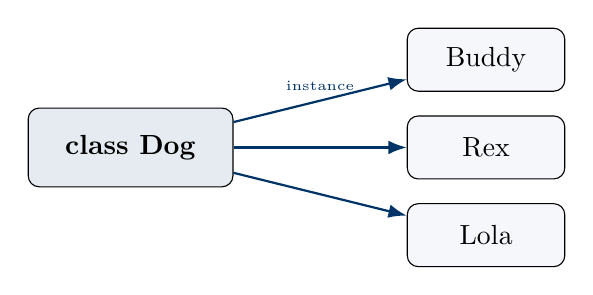
\begin{tikzpicture}[node distance=1.5cm, >=Latex]
  \node[draw,rounded corners,fill=PrimaryBlue!10,minimum width=2.6cm,minimum height=1.0cm] (cls) {\textbf{class Dog}};
  \node[draw,rounded corners,fill=LightGray,minimum width=2.0cm,minimum height=0.8cm,right=2.2cm of cls] (o1) {Rex};
  \node[draw,rounded corners,fill=LightGray,minimum width=2.0cm,minimum height=0.8cm,below=0.3cm of o1] (o2) {Lola};
  \node[draw,rounded corners,fill=LightGray,minimum width=2.0cm,minimum height=0.8cm,above=0.3cm of o1] (o3) {Buddy};
  \draw[->,thick,PrimaryBlue] (cls) -- node[above,font=\tiny]{instance} (o3);
  \draw[->,thick,PrimaryBlue] (cls) -- (o1);
  \draw[->,thick,PrimaryBlue] (cls) -- (o2);
\end{tikzpicture}
\end{center}

\vspace{0.1cm}
\begin{tcolorbox}[lecturebox,title=Key idea]
The \keyword{class} describes structure and behavior once. Each \keyword{object} carries its own data but shares the same behavior defined by its class.
\end{tcolorbox}
\end{frame}


\begin{frame}[fragile]
\frametitle{The class Keyword}
\small
We define a class with \codeword{class}. By convention, class names use \keyword{CapWords}.

\vspace{0.15cm}
\begin{lstlisting}[style=pycode]
class Dog:
    """A simple Dog class."""
    species = "Canis familiaris"      # class variable

    def __init__(self, name, age):    # constructor
        self.name = name              # instance variable
        self.age  = age

    def bark(self):                   # instance method
        return f"{self.name} says woof!"

rex = Dog("Rex", 5)         # create an instance
print(rex.bark())           # Rex says woof!
print(rex.species)          # Canis familiaris
\end{lstlisting}

\begin{tcolorbox}[lecturebox,title=Vocabulary]
\begin{itemize}\setlength\itemsep{0.05cm}
  \item \keyword{Class}: \texttt{Dog}, the blueprint.
  \item \keyword{Instance}: \texttt{rex}, a specific dog created from the blueprint.
  \item \keyword{Attribute}: a piece of data on the class or instance (e.g.\ \texttt{name}).
  \item \keyword{Method}: a function defined inside a class.
\end{itemize}
\end{tcolorbox}
\end{frame}


\begin{frame}[fragile]
\frametitle{The \_\_init\_\_ Constructor and self}
\small
The \codeword{\_\_init\_\_} method runs \keyword{automatically} every time a new object is created. Its job is to set up the instance's starting state.

\vspace{0.1cm}
\begin{lstlisting}[style=pycode]
class Point:
    def __init__(self, x, y):
        self.x = x      # bind data to THIS instance
        self.y = y

p1 = Point(1, 2)        # Python calls Point.__init__(p1, 1, 2)
p2 = Point(5, 7)
print(p1.x, p2.x)       # 1 5  -> independent state
\end{lstlisting}

\begin{columns}[T,totalwidth=0.96\textwidth]
\begin{column}{0.5\textwidth}
\begin{tcolorbox}[lecturebox,title=What is self?]
\codeword{self} is the \keyword{instance being worked on}. Python passes it as the first argument behind the scenes. It is not a keyword, only a strong convention.
\end{tcolorbox}
\end{column}
\begin{column}{0.46\textwidth}
\begin{tcolorbox}[lecturebox,title=Common mistake]
Forgetting \codeword{self} as the first parameter is the number-one beginner error in Python OOP.
\end{tcolorbox}
\end{column}
\end{columns}
\end{frame}


\begin{frame}[fragile]
\frametitle{Instance Variables vs. Class Variables}
\small
\begin{columns}[T,totalwidth=0.96\textwidth]
\begin{column}{0.48\textwidth}
\textbf{Class variable}
\begin{itemize}\setlength\itemsep{0.04cm}
  \item Defined directly inside the class.
  \item \keyword{Shared} by every instance.
  \item Stored in the class itself.
\end{itemize}
\end{column}
\begin{column}{0.48\textwidth}
\textbf{Instance variable}
\begin{itemize}\setlength\itemsep{0.04cm}
  \item Defined inside \codeword{\_\_init\_\_} (or other methods).
  \item \keyword{Unique} to each instance.
  \item Stored in the instance itself.
\end{itemize}
\end{column}
\end{columns}

\vspace{0.18cm}
\begin{lstlisting}[style=pycode]
class Counter:
    total = 0                        # CLASS variable (shared)

    def __init__(self, name):
        self.name = name             # INSTANCE variable
        Counter.total += 1

a = Counter("A")
b = Counter("B")
print(Counter.total)                 # 2  -> shared across all
\end{lstlisting}

\begin{bluebox}{Rule of thumb}
Use class variables for values that belong to the type as a whole. Use instance variables for values that belong to a specific object.
\end{bluebox}
\end{frame}


\begin{frame}[fragile]
\frametitle{Class vs. Instance Namespaces}
\small
Every class and every instance has its own namespace (a dictionary of names). Python looks up an attribute first on the instance, then on the class.

\vspace{0.12cm}
\begin{lstlisting}[style=pycode]
class Dog:
    legs = 4                  # class namespace

rex = Dog()
print(rex.legs)               # 4  -> looked up on the class
rex.legs = 3                  # creates an INSTANCE attribute
print(rex.legs)               # 3  -> from instance namespace
print(Dog.legs)               # 4  -> the class is unchanged

print(rex.__dict__)           # {'legs': 3}
print(Dog.__dict__.keys())    # dict_keys([..., 'legs', ...])
\end{lstlisting}

\begin{tcolorbox}[lecturebox,title=Mental model]
Setting \codeword{rex.legs = 3} does \keyword{not} mutate the class. It adds a new key to the instance's own \codeword{\_\_dict\_\_}, which then shadows the class attribute for this instance only.
\end{tcolorbox}
\end{frame}


\begin{frame}[fragile]
\frametitle{Object Identity: id(), is, and ==}
\small
Python distinguishes between two objects being the \keyword{same object} and two objects having \keyword{equal values}.

\vspace{0.1cm}
\renewcommand{\arraystretch}{1.25}
\begin{tabularx}{\linewidth}{>{\bfseries}p{2.0cm}X}
\toprule
Operator / function & Meaning \\
\midrule
\code{id(x)} & A unique integer for the object (its identity). \\
\code{a is b} & True when \texttt{a} and \texttt{b} are the \keyword{same} object. \\
\code{a == b} & True when \texttt{a} and \texttt{b} have \keyword{equal} values. Calls \codeword{\_\_eq\_\_}. \\
\bottomrule
\end{tabularx}

\vspace{0.18cm}
\begin{lstlisting}[style=pycode]
a = [1, 2, 3]
b = [1, 2, 3]
c = a

a == b      # True   -> same value
a is b      # False  -> different objects
a is c      # True   -> same object (alias)
\end{lstlisting}

\begin{bluebox}{Practical rule}
Use \codeword{is} only when comparing with \codeword{None}, \codeword{True}, or \codeword{False}. For everything else, use \codeword{==}.
\end{bluebox}
\end{frame}


\begin{frame}[fragile]
\frametitle{Representing Objects: \_\_str\_\_ vs. \_\_repr\_\_}
\small
Python uses two methods to convert an object to text. They have different audiences.

\vspace{0.12cm}
\begin{columns}[T,totalwidth=0.96\textwidth]
\begin{column}{0.48\textwidth}
\textbf{\codeword{\_\_str\_\_}}
\begin{itemize}\setlength\itemsep{0.04cm}
  \item Used by \codeword{print()} and \codeword{str()}.
  \item For \keyword{end users}: friendly and short.
\end{itemize}
\end{column}
\begin{column}{0.48\textwidth}
\textbf{\codeword{\_\_repr\_\_}}
\begin{itemize}\setlength\itemsep{0.04cm}
  \item Used in the REPL and by \codeword{repr()}.
  \item For \keyword{developers}: precise and unambiguous.
\end{itemize}
\end{column}
\end{columns}

\vspace{0.18cm}
\begin{lstlisting}[style=pycode]
class Point:
    def __init__(self, x, y):
        self.x, self.y = x, y
    def __repr__(self):
        return f"Point(x={self.x}, y={self.y})"
    def __str__(self):
        return f"({self.x}, {self.y})"

p = Point(3, 4)
print(p)         # (3, 4)              -> __str__
print(repr(p))   # Point(x=3, y=4)     -> __repr__
[p]              # [Point(x=3, y=4)]   -> repr inside containers
\end{lstlisting}
\end{frame}


% ============================================================
% MODULE 2 TITLE SLIDE
% ============================================================
\begin{noheadline}
\begin{frame}
\frametitle{Module 2: METHODS, PROPERTIES \& ENCAPSULATION}
\vspace{1.2cm}
\begin{center}
  {\fontsize{30}{36}\selectfont\textbf{Module 2}}\\[0.35cm]
  {\fontsize{18}{22}\selectfont METHODS, PROPERTIES \& ENCAPSULATION}\\[0.7cm]
  \tcbox[colback=PrimaryBlue!6,colframe=PrimaryBlue,arc=3mm,boxrule=1pt,left=8mm,right=8mm,top=4mm,bottom=4mm,fontupper=\Large]{Methods, properties, privacy, and memory}
\end{center}
\end{frame}
\end{noheadline}


% ============================================================
% MODULE 2 CONTENT SLIDE
% ============================================================
\begin{frame}
\frametitle{Module Content}
\small
This module covers how objects expose and protect their data through methods, properties, and privacy conventions.

\vspace{0.16cm}
\begin{columns}[T,totalwidth=0.96\textwidth]
\begin{column}{0.48\textwidth}
\begin{itemize}\setlength\itemsep{0.08cm}
  \item \keyword{Three kinds of methods}: instance, class, and static.
  \item \keyword{Properties}: using \codeword{@property} for computed and validated attributes.
  \item \keyword{Read-only attributes}: preventing external modification.
\end{itemize}
\end{column}
\begin{column}{0.48\textwidth}
\begin{itemize}\setlength\itemsep{0.08cm}
  \item \keyword{Privacy conventions}: single \codeword{\_} vs.\ double \codeword{\_\_} name mangling.
  \item \keyword{\_\_slots\_\_}: restricting attributes for memory optimization.
\end{itemize}
\end{column}
\end{columns}
\end{frame}


% ============================================================
% 4.2 ATTRIBUTES AND METHODS
% ============================================================
\begin{frame}[fragile]
\frametitle{Three Kinds of Methods}
\small
A class can hold three kinds of methods. They differ in what is automatically passed as the first argument.

\vspace{0.12cm}
\begin{lstlisting}[style=pycode]
class Pizza:
    radius_cm = 30                       # class attribute

    def __init__(self, toppings):
        self.toppings = toppings

    def describe(self):                  # INSTANCE method
        return f"Pizza with {self.toppings}"

    @classmethod
    def margherita(cls):                 # CLASS method (factory)
        return cls(["mozzarella", "tomato", "basil"])

    @staticmethod
    def is_round():                      # STATIC method
        return True
\end{lstlisting}

\begin{itemize}\setlength\itemsep{0.04cm}
  \item \keyword{Instance method}: receives \codeword{self}; works on a single object.
  \item \keyword{Class method}: receives \codeword{cls}; often used as an alternative constructor.
  \item \keyword{Static method}: receives nothing extra; a plain function placed inside the class for grouping.
\end{itemize}
\end{frame}


\begin{frame}[fragile]
\frametitle{Properties: @property}
\small
A \keyword{property} lets you compute or validate an attribute, while keeping the simple \codeword{object.attribute} syntax.

\vspace{0.12cm}
\begin{lstlisting}[style=pycode]
class Circle:
    def __init__(self, radius):
        self._radius = radius

    @property
    def radius(self):                  # getter
        return self._radius

    @radius.setter
    def radius(self, value):           # setter with validation
        if value < 0:
            raise ValueError("radius must be >= 0")
        self._radius = value

    @property
    def area(self):                    # computed, read-only
        return 3.14159 * self._radius ** 2

c = Circle(5)
print(c.area)            # 78.5  (no parentheses!)
c.radius = 10            # validated through the setter
\end{lstlisting}
\end{frame}


\begin{frame}[fragile]
\frametitle{Read-only Attributes}
\small
If you omit the setter, the property becomes \keyword{read-only} from outside the class.

\vspace{0.15cm}
\begin{lstlisting}[style=pycode]
class User:
    def __init__(self, username):
        self._username = username

    @property
    def username(self):
        return self._username        # no setter -> read-only

u = User("alice")
print(u.username)                    # alice
u.username = "bob"                   # AttributeError
\end{lstlisting}

\begin{tcolorbox}[lecturebox,title=Pythonic principle]
Start with a plain attribute. Switch to a property \keyword{only when you need} validation, computation, or read-only behavior. The caller's syntax does not change, so this refactor is invisible from outside.
\end{tcolorbox}
\end{frame}


\begin{frame}[fragile]
\frametitle{Privacy Conventions: \_ vs. \_\_}
\small
Python has \keyword{no truly private} attributes. It uses naming conventions instead.

\vspace{0.12cm}
\begin{lstlisting}[style=pycode]
class Account:
    def __init__(self, balance):
        self.owner    = "public"     # public attribute
        self._balance = balance      # "internal use only"
        self.__pin    = 1234         # name-mangled by Python

a = Account(500)
a._balance        # works, but you are saying "I know I shouldn't"
a.__pin           # AttributeError
a._Account__pin   # 1234   -> the actual mangled name
\end{lstlisting}

\renewcommand{\arraystretch}{1.25}
\begin{tabularx}{\linewidth}{>{\bfseries}p{2.0cm}X}
\toprule
Convention & Meaning \\
\midrule
\code{name}        & Public attribute. Free to use. \\
\code{\_name}      & ``Internal, hands-off.'' Linters warn but Python does not enforce. \\
\code{\_\_name}    & \keyword{Name-mangled} to \codeword{\_ClassName\_\_name}. Used to avoid clashes in subclasses, not for security. \\
\bottomrule
\end{tabularx}
\end{frame}


\begin{frame}[fragile]
\frametitle{\_\_slots\_\_: Memory Optimization}
\small
By default, every instance carries a \codeword{\_\_dict\_\_}. \codeword{\_\_slots\_\_} replaces this dictionary with a fixed array of attribute slots.

\vspace{0.15cm}
\begin{columns}[T,totalwidth=0.98\textwidth]
\begin{column}{0.55\textwidth}
\begin{lstlisting}[style=pycodesmall]
class PointSlow:
    def __init__(self, x, y):
        self.x = x
        self.y = y

class PointFast:
    __slots__ = ("x", "y")
    def __init__(self, x, y):
        self.x = x
        self.y = y

p = PointFast(1, 2)
p.z = 3   # AttributeError: only x, y allowed
\end{lstlisting}
\end{column}
\begin{column}{0.42\textwidth}
\textbf{Pros}
\begin{itemize}\setlength\itemsep{0.02cm}
  \item Smaller memory (40--50\% less per instance).
  \item Faster attribute access.
\end{itemize}
\vspace{0.12cm}
\textbf{Cons}
\begin{itemize}\setlength\itemsep{0.02cm}
  \item No new attributes after definition.
  \item Multiple inheritance becomes trickier.
\end{itemize}
\end{column}
\end{columns}

\vspace{0.15cm}
\begin{bluebox}{When to use}
Reach for \codeword{\_\_slots\_\_} when you create \keyword{millions} of small objects. For typical app code it is rarely needed.
\end{bluebox}
\end{frame}


% ============================================================
% MODULE 3 TITLE SLIDE
% ============================================================
\begin{noheadline}
\begin{frame}
\frametitle{Module 3: INHERITANCE \& POLYMORPHISM}
\vspace{1.2cm}
\begin{center}
  {\fontsize{30}{36}\selectfont\textbf{Module 3}}\\[0.35cm]
  {\fontsize{25}{30}\selectfont INHERITANCE \& POLYMORPHISM}\\[0.7cm]
  \tcbox[colback=PrimaryBlue!6,colframe=PrimaryBlue,arc=3mm,boxrule=1pt,left=8mm,right=8mm,top=4mm,bottom=4mm,fontupper=\Large]{Class hierarchies, duck typing, and mixins}
\end{center}
\end{frame}
\end{noheadline}


% ============================================================
% MODULE 3 CONTENT SLIDE
% ============================================================
\begin{frame}
\frametitle{Module Content}
\small
This module covers building class hierarchies and writing flexible code that works across related types.

\vspace{0.16cm}
\begin{columns}[T,totalwidth=0.96\textwidth]
\begin{column}{0.48\textwidth}
\begin{itemize}\setlength\itemsep{0.08cm}
  \item \keyword{Single inheritance}: extending a class with \codeword{super()}.
  \item \keyword{MRO}: Python's method resolution order (C3 linearisation).
  \item \keyword{Multiple inheritance}: the diamond problem and how Python resolves it.
  \item \keyword{Abstract base classes}: enforcing interface contracts.
\end{itemize}
\end{column}
\begin{column}{0.48\textwidth}
\begin{itemize}\setlength\itemsep{0.08cm}
  \item \keyword{Polymorphism}: writing code that works for any compatible type.
  \item \keyword{Duck typing}: if it walks like a duck\ldots
  \item \keyword{Mixins}: adding orthogonal behaviour through inheritance.
  \item \keyword{Type checking}: \codeword{isinstance()} and \codeword{issubclass()}.
\end{itemize}
\end{column}
\end{columns}
\end{frame}


% ============================================================
% 4.3 INHERITANCE AND POLYMORPHISM
% ============================================================
\begin{frame}[fragile]
\frametitle{Single Inheritance and super()}
\small
A \keyword{child class} reuses behavior from a \keyword{parent class} and may add or override methods.

\vspace{0.1cm}
\begin{lstlisting}[style=pycode]
class Animal:
    def __init__(self, name):
        self.name = name
    def speak(self):
        return "Some sound"

class Dog(Animal):                       # Dog INHERITS from Animal
    def __init__(self, name, breed):
        super().__init__(name)           # call parent's __init__
        self.breed = breed
    def speak(self):                     # OVERRIDE
        return f"{self.name} barks!"

d = Dog("Rex", "Labrador")
print(d.speak())                         # Rex barks!
print(isinstance(d, Animal))             # True
\end{lstlisting}

\begin{bluebox}{Why super()?}
\codeword{super()} delegates to the next class in the lookup order. It is safer than naming the parent directly, especially when classes are later reorganized.
\end{bluebox}
\end{frame}


\begin{frame}[fragile]
\frametitle{Method Resolution Order (MRO)}
\small
When a method is called, Python searches classes in a specific order called the \keyword{Method Resolution Order}. It uses the \keyword{C3 linearization} algorithm.

\vspace{0.15cm}
\begin{columns}[T,totalwidth=0.96\textwidth]
\begin{column}{0.5\textwidth}
\begin{lstlisting}[style=pycode]
class A: pass
class B(A): pass
class C(A): pass
class D(B, C): pass

print(D.__mro__)
# (D, B, C, A, object)
\end{lstlisting}
\end{column}
\begin{column}{0.46\textwidth}
\begin{tcolorbox}[lecturebox,title=Two C3 guarantees]
\begin{itemize}\setlength\itemsep{0.05cm}
  \item A subclass appears \keyword{before} its parents.
  \item The relative order of parents is preserved.
\end{itemize}
\end{tcolorbox}
\end{column}
\end{columns}

\vspace{0.15cm}
\begin{tcolorbox}[lecturebox,title=Inspecting the MRO]
Use \codeword{ClassName.\_\_mro\_\_} or \codeword{ClassName.mro()} to see the exact lookup order. Every \codeword{super()} call follows this list.
\end{tcolorbox}
\end{frame}


\begin{frame}[fragile]
\frametitle{Multiple Inheritance and the Diamond Problem}
\small
A class can inherit from more than one parent. When two parents share a common ancestor, we get a \keyword{diamond} shape.

\vspace{0.1cm}
\begin{columns}[T,totalwidth=0.96\textwidth]
\begin{column}{0.36\textwidth}
\begin{center}
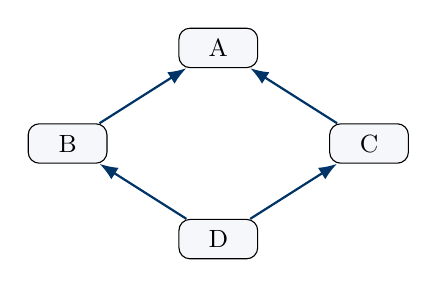
\begin{tikzpicture}[node distance=0.7cm and 0.9cm,
    every node/.style={draw,rectangle,rounded corners,fill=LightGray,
                       minimum width=1.0cm,minimum height=0.5cm,font=\small}]
    \node (A) {A};
    \node (B) [below left=of A]  {B};
    \node (C) [below right=of A] {C};
    \node (D) [below right=of B] {D};
    \draw[-Latex,PrimaryBlue,thick] (B) -- (A);
    \draw[-Latex,PrimaryBlue,thick] (C) -- (A);
    \draw[-Latex,PrimaryBlue,thick] (D) -- (B);
    \draw[-Latex,PrimaryBlue,thick] (D) -- (C);
\end{tikzpicture}
\end{center}
\end{column}
\begin{column}{0.60\textwidth}
\begin{lstlisting}[style=pycodesmall]
class A:
    def hi(self): print("A")
class B(A):
    def hi(self): print("B"); super().hi()
class C(A):
    def hi(self): print("C"); super().hi()
class D(B, C):
    def hi(self): print("D"); super().hi()

D().hi()       # D B C A
\end{lstlisting}
\end{column}
\end{columns}

\begin{bluebox}{What C3 prevents}
Without a careful algorithm, calling \codeword{D().hi()} could call \texttt{A} twice or skip a class entirely. C3 produces a single, predictable order: \texttt{D, B, C, A}.
\end{bluebox}
\end{frame}


\begin{frame}[fragile]
\frametitle{Abstract Base Classes}
\small
An \keyword{abstract base class} (ABC) declares methods that subclasses \keyword{must} implement.

\vspace{0.05cm}
\begin{lstlisting}[style=pycodesmall]
from abc import ABC, abstractmethod

class Shape(ABC):
    @abstractmethod
    def area(self):
        ...
    @abstractmethod
    def perimeter(self):
        ...

class Square(Shape):
    def __init__(self, side):
        self.side = side
    def area(self):       return self.side ** 2
    def perimeter(self):  return 4 * self.side

Shape()                  # TypeError: can't instantiate abstract class
print(Square(3).area())  # 9
\end{lstlisting}

\begin{tcolorbox}[lecturebox,title=Why use abstract classes?]
They make the \keyword{contract} explicit. Anyone subclassing \texttt{Shape} is forced to provide \codeword{area} and \codeword{perimeter}, so the rest of the program can rely on them.
\end{tcolorbox}
\end{frame}


\begin{frame}[fragile]
\frametitle{Polymorphism and Duck Typing}
\small
\keyword{Polymorphism} means the same call works on different types. Python takes the loose, flexible version called \keyword{duck typing}.

\vspace{0.12cm}
\begin{lstlisting}[style=pycode]
class Duck:
    def speak(self): return "Quack"
class Robot:
    def speak(self): return "Beep"
class Cat:
    def speak(self): return "Meow"

def chorus(creatures):
    for c in creatures:           # don't care about the type
        print(c.speak())          # only the interface matters

chorus([Duck(), Robot(), Cat()])
\end{lstlisting}

\begin{bluebox}{The Pythonic credo}
``If it walks like a duck and quacks like a duck, it is a duck.'' Java and C++ require a shared base class. Python just calls \codeword{.speak()} and trusts you.
\end{bluebox}
\end{frame}


\begin{frame}[fragile]
\frametitle{Mixins: Composition through Inheritance}
\small
A \keyword{mixin} is a small class meant to be combined with others to add a focused piece of behavior.

\vspace{0.1cm}
\begin{lstlisting}[style=pycode]
class JSONMixin:
    def to_json(self):
        import json
        return json.dumps(self.__dict__)

class TimestampMixin:
    def stamp(self):
        from datetime import datetime
        self.created_at = datetime.now()

class User(JSONMixin, TimestampMixin):
    def __init__(self, name):
        self.name = name
        self.stamp()

u = User("Ada")
print(u.to_json())
\end{lstlisting}

\begin{tcolorbox}[lecturebox,title=Where you have seen this]
Mixins are used heavily in \keyword{Django} (e.g.\ \codeword{LoginRequiredMixin}) and in \keyword{Keras} training-loop classes. Each mixin contributes one orthogonal feature.
\end{tcolorbox}
\end{frame}


\begin{frame}[fragile]
\frametitle{Type Checking: isinstance() and issubclass()}
\small
\codeword{isinstance(obj, T)} checks whether an object is of type \texttt{T} (or a subclass). \codeword{issubclass(C, P)} checks whether one class inherits from another.

\vspace{0.12cm}
\begin{lstlisting}[style=pycode]
isinstance(5, int)               # True
isinstance(5, (int, float))      # True   -> tuple of types
isinstance(True, int)            # True   -> bool IS an int!

issubclass(bool, int)            # True
issubclass(Dog, Animal)          # True
\end{lstlisting}

\begin{bluebox}{Use sparingly}
Heavy use of \codeword{isinstance} often signals you should be using \keyword{polymorphism} instead. Reserve type checks for boundaries: input validation, dispatching, and library entry points.
\end{bluebox}
\end{frame}


% ============================================================
% MODULE 4 TITLE SLIDE
% ============================================================
\begin{noheadline}
\begin{frame}
\frametitle{Module 4: OOP DESIGN PRINCIPLES}
\vspace{1.2cm}
\begin{center}
  {\fontsize{30}{36}\selectfont\textbf{Module 4}}\\[0.35cm]
  {\fontsize{25}{30}\selectfont OOP DESIGN PRINCIPLES}\\[0.7cm]
  \tcbox[colback=PrimaryBlue!6,colframe=PrimaryBlue,arc=3mm,boxrule=1pt,left=8mm,right=8mm,top=4mm,bottom=4mm,fontupper=\Large]{Encapsulation, SOLID, composition, and dataclasses}
\end{center}
\end{frame}
\end{noheadline}


% ============================================================
% MODULE 4 CONTENT SLIDE
% ============================================================
\begin{frame}
\frametitle{Module Content}
\small
This module covers industry best practices for writing clean, extensible, and maintainable object-oriented code.

\vspace{0.16cm}
\begin{columns}[T,totalwidth=0.96\textwidth]
\begin{column}{0.48\textwidth}
\begin{itemize}\setlength\itemsep{0.08cm}
  \item \keyword{Encapsulation}: hiding the ``how'' behind a clean interface.
  \item \keyword{SOLID principles}: an overview of the five design guidelines.
  \item \keyword{Composition over inheritance}: favouring has-a over is-a.
\end{itemize}
\end{column}
\begin{column}{0.48\textwidth}
\begin{itemize}\setlength\itemsep{0.08cm}
  \item \keyword{Dataclasses}: eliminating boilerplate with \codeword{@dataclass}.
  \item \keyword{Named tuples vs.\ dataclasses}: choosing the right data container.
\end{itemize}
\end{column}
\end{columns}
\end{frame}


% ============================================================
% 4.4 ENCAPSULATION AND DESIGN PRINCIPLES
% ============================================================
\begin{frame}[fragile]
\frametitle{Encapsulation: Hiding the ``How''}
\small
\keyword{Encapsulation} means exposing \keyword{what} an object does, while hiding \keyword{how} it does it.

\vspace{0.18cm}
\begin{columns}[T,totalwidth=0.96\textwidth]
\begin{column}{0.5\textwidth}
\begin{itemize}\setlength\itemsep{0.06cm}
  \item Keep internal state behind \texttt{\_} or properties.
  \item Offer a stable public interface.
  \item Validate, log, or cache transparently inside setters.
  \item Refactor internals freely without breaking callers.
\end{itemize}
\end{column}
\begin{column}{0.46\textwidth}
\begin{tcolorbox}[lecturebox,title=Self-test]
Could I rewrite the internals of this class tomorrow without changing any of its callers?

\vspace{0.05cm}
If yes, the class is well-encapsulated.
\end{tcolorbox}
\end{column}
\end{columns}

\vspace{0.1cm}
\begin{bluebox}{Key idea}
Encapsulation is the discipline behind every other principle in this section. It is what lets us change code with confidence.
\end{bluebox}
\end{frame}


\begin{frame}[fragile]
\frametitle{SOLID Principles (Overview)}
\small
\keyword{SOLID} is a set of five design principles for writing maintainable object-oriented code.

\vspace{0.15cm}
\renewcommand{\arraystretch}{1.30}
\begin{tabularx}{\linewidth}{>{\bfseries}p{4.4cm}X}
\toprule
Principle & In one sentence \\
\midrule
S --- Single Responsibility & A class should have \keyword{one} reason to change. \\
O --- Open/Closed           & Code should be open for \keyword{extension}, closed for \keyword{modification}. \\
L --- Liskov Substitution   & A subclass must be usable wherever its parent is expected. \\
I --- Interface Segregation & Many small interfaces beat one fat interface. \\
D --- Dependency Inversion  & Depend on abstractions, not on concrete implementations. \\
\bottomrule
\end{tabularx}

\vspace{0.18cm}
\begin{tcolorbox}[lecturebox,title=Today's focus]
We focus on the first two: \keyword{S} (each class has one job) and \keyword{O} (extend by subclassing or composing, do not edit working code). The other three are explored in larger software-engineering courses.
\end{tcolorbox}
\end{frame}


\begin{frame}[fragile]
\frametitle{Composition over Inheritance}
\small
\keyword{Inheritance} models an \keyword{is-a} relationship. \keyword{Composition} models a \keyword{has-a} relationship.

\vspace{0.12cm}
\begin{lstlisting}[style=pycode]
# Inheritance can become rigid
class FlyingCar(Car, Plane):
    ...

# Composition is flexible: a Car HAS an engine and HAS wheels
class Engine:
    def start(self): ...
class Wheels:
    def roll(self):  ...

class Car:
    def __init__(self):
        self.engine = Engine()
        self.wheels = Wheels()
    def drive(self):
        self.engine.start()
        self.wheels.roll()
\end{lstlisting}

\begin{tcolorbox}[lecturebox,title=Why prefer composition]
Easier to test, easier to swap parts, and easier to extend. Use inheritance only when there is a genuine \keyword{is-a} relationship.
\end{tcolorbox}
\end{frame}


\begin{frame}[fragile]
\frametitle{Dataclasses: Boilerplate-free Classes}
\small
The \codeword{@dataclass} decorator generates \codeword{\_\_init\_\_}, \codeword{\_\_repr\_\_}, and \codeword{\_\_eq\_\_} for you, based on type-annotated fields.

\vspace{0.12cm}
\begin{lstlisting}[style=pycode]
from dataclasses import dataclass, field

@dataclass
class Product:
    name: str
    price: float
    tags: list = field(default_factory=list)
    in_stock: bool = True

p = Product("Book", 19.99)
print(p)
# Product(name='Book', price=19.99, tags=[], in_stock=True)

p == Product("Book", 19.99)         # True   -> auto __eq__
\end{lstlisting}

\begin{bluebox}{Useful flags}
\codeword{frozen=True} makes instances immutable. \codeword{order=True} adds comparison operators. \codeword{slots=True} (Python 3.10+) adds \codeword{\_\_slots\_\_} automatically.
\end{bluebox}
\end{frame}


\begin{frame}[fragile]
\frametitle{Named Tuples vs. Dataclasses}
\small
Both build small data containers. They differ in mutability and flexibility.

\vspace{0.12cm}
\begin{columns}[T,totalwidth=0.98\textwidth]
\begin{column}{0.48\textwidth}
\textbf{NamedTuple}
\begin{lstlisting}[style=pycodesmall]
from typing import NamedTuple

class Point(NamedTuple):
    x: float
    y: float

p = Point(1, 2)
p[0]      # tuple-like access
p.x       # attribute access
# IMMUTABLE, hashable
\end{lstlisting}
\end{column}
\begin{column}{0.48\textwidth}
\textbf{Dataclass}
\begin{lstlisting}[style=pycodesmall]
from dataclasses import dataclass

@dataclass
class Point:
    x: float
    y: float

p = Point(1, 2)
p.x = 5     # mutable by default
# Add methods freely
\end{lstlisting}
\end{column}
\end{columns}

\vspace{0.1cm}
\begin{tcolorbox}[lecturebox,title=Choosing the right tool]
\begin{itemize}\setlength\itemsep{0.04cm}
  \item Pick \keyword{NamedTuple} for small, immutable, tuple-like records.
  \item Pick \keyword{dataclass} when you need mutability, defaults, or extra methods.
\end{itemize}
\end{tcolorbox}
\end{frame}


% ============================================================
% MODULE 5 TITLE SLIDE
% ============================================================
\begin{noheadline}
\begin{frame}
\frametitle{Module 5: MAGIC METHODS \& INTROSPECTION}
\vspace{1.2cm}
\begin{center}
  {\fontsize{30}{36}\selectfont\textbf{Module 5}}\\[0.35cm]
  {\fontsize{22}{28}\selectfont MAGIC METHODS \& INTROSPECTION}\\[0.7cm]
  \tcbox[colback=PrimaryBlue!6,colframe=PrimaryBlue,arc=3mm,boxrule=1pt,left=8mm,right=8mm,top=4mm,bottom=4mm,fontupper=\Large]{Dunders, operator overloading, and runtime inspection}
\end{center}
\end{frame}
\end{noheadline}


% ============================================================
% MODULE 5 CONTENT SLIDE
% ============================================================
\begin{frame}
\frametitle{Module Content}
\small
This module unlocks Python's operator overloading system and covers inspecting objects at runtime.

\vspace{0.16cm}
\begin{columns}[T,totalwidth=0.96\textwidth]
\begin{column}{0.48\textwidth}
\begin{itemize}\setlength\itemsep{0.08cm}
  \item \keyword{Dunder methods}: how Python calls them automatically with built-in syntax.
  \item \keyword{Arithmetic dunders}: \codeword{\_\_add\_\_}, \codeword{\_\_mul\_\_}, and friends.
  \item \keyword{Comparison dunders}: \codeword{\_\_eq\_\_}, \codeword{\_\_lt\_\_}, and total ordering.
  \item \keyword{Container dunders}: \codeword{\_\_len\_\_}, \codeword{\_\_getitem\_\_}, and iteration.
\end{itemize}
\end{column}
\begin{column}{0.48\textwidth}
\begin{itemize}\setlength\itemsep{0.08cm}
  \item \keyword{Context manager dunders}: \codeword{\_\_enter\_\_} and \codeword{\_\_exit\_\_}.
  \item \keyword{Callable objects}: \codeword{\_\_call\_\_}.
  \item \keyword{Introspection}: \codeword{\_\_dict\_\_}, \codeword{\_\_class\_\_}, and \codeword{\_\_slots\_\_}.
  \item \keyword{Worked example}: building a Matrix class end-to-end.
\end{itemize}
\end{column}
\end{columns}
\end{frame}


% ============================================================
% 4.5 MAGIC (DUNDER) METHODS
% ============================================================
\begin{frame}[fragile]
\frametitle{Magic Methods (Dunders)}
\small
\keyword{Dunder methods} are methods with double-underscore names. Python calls them automatically when you use built-in syntax. Implementing them makes your class \keyword{feel like a built-in type}.

\vspace{0.15cm}
\renewcommand{\arraystretch}{1.25}
\begin{tabularx}{\linewidth}{>{\bfseries}p{3.0cm}X}
\toprule
Syntax you write & Method Python calls \\
\midrule
\code{a + b}              & \codeword{a.\_\_add\_\_(b)} \\
\code{a == b}             & \codeword{a.\_\_eq\_\_(b)} \\
\code{len(a)}             & \codeword{a.\_\_len\_\_()} \\
\code{a[i]}               & \codeword{a.\_\_getitem\_\_(i)} \\
\code{for x in a}         & \codeword{a.\_\_iter\_\_()} \\
\code{a()}                & \codeword{a.\_\_call\_\_()} \\
\code{with a:}            & \codeword{a.\_\_enter\_\_} / \codeword{\_\_exit\_\_} \\
\bottomrule
\end{tabularx}
\end{frame}


\begin{frame}[fragile]
\frametitle{Arithmetic Dunders}
\small
Define arithmetic dunders to use \codeword{+}, \codeword{-}, \codeword{*}, \codeword{/}, and \codeword{**} on your objects.

\vspace{0.12cm}
\begin{lstlisting}[style=pycode]
class Vector:
    def __init__(self, x, y):
        self.x, self.y = x, y
    def __add__(self, o):     return Vector(self.x + o.x, self.y + o.y)
    def __sub__(self, o):     return Vector(self.x - o.x, self.y - o.y)
    def __mul__(self, k):     return Vector(self.x * k,   self.y * k)
    def __truediv__(self, k): return Vector(self.x / k,   self.y / k)
    def __pow__(self, n):     return Vector(self.x ** n,  self.y ** n)
    def __repr__(self):       return f"Vector({self.x}, {self.y})"

v = Vector(1, 2) + Vector(3, 4)      # Vector(4, 6)
w = Vector(2, 3) * 5                 # Vector(10, 15)
\end{lstlisting}

\begin{bluebox}{Reflected operations}
For \codeword{5 * v} (where \texttt{v} is a Vector), Python tries \codeword{int.\_\_mul\_\_} first, then falls back to \codeword{Vector.\_\_rmul\_\_}. Define the reflected versions when needed.
\end{bluebox}
\end{frame}


\begin{frame}[fragile]
\frametitle{Comparison Dunders}
\small
Comparison dunders make your objects work with \codeword{<}, \codeword{<=}, \codeword{==}, \codeword{>=}, \codeword{>}, and with \codeword{sorted()}.

\vspace{0.12cm}
\begin{lstlisting}[style=pycode]
from functools import total_ordering

@total_ordering
class Money:
    def __init__(self, amount):
        self.amount = amount
    def __eq__(self, o):
        return self.amount == o.amount
    def __lt__(self, o):
        return self.amount < o.amount
    # __le__, __gt__, __ge__ filled in by @total_ordering

a, b = Money(10), Money(20)
print(a < b)      # True
print(a >= b)     # False
print(sorted([Money(30), Money(10), Money(20)]))
\end{lstlisting}

\begin{tcolorbox}[lecturebox,title=Tip]
Implement \codeword{\_\_eq\_\_} and \codeword{\_\_lt\_\_}, then let \codeword{@total\_ordering} fill in the rest. You write less code and get consistent behavior.
\end{tcolorbox}
\end{frame}


\begin{frame}[fragile]
\frametitle{Container Dunders}
\small
Implementing container dunders makes your class behave like a list, dict, or set.

\vspace{0.1cm}
\begin{lstlisting}[style=pycode]
class Playlist:
    def __init__(self, songs):     self.songs = list(songs)
    def __len__(self):             return len(self.songs)
    def __getitem__(self, i):      return self.songs[i]
    def __setitem__(self, i, v):   self.songs[i] = v
    def __delitem__(self, i):      del self.songs[i]
    def __contains__(self, s):     return s in self.songs
    def __iter__(self):            return iter(self.songs)

pl = Playlist(["A", "B", "C"])
len(pl)                # 3
pl[0]                  # 'A'
"B" in pl              # True
for song in pl:        # iterates
    print(song)
\end{lstlisting}

\begin{bluebox}{The pattern}
Decide which built-in operations make sense for your class, then implement the matching dunders. Users get a familiar, Pythonic interface for free.
\end{bluebox}
\end{frame}


\begin{frame}[fragile]
\frametitle{Context Manager Dunders}
\small
\codeword{\_\_enter\_\_} and \codeword{\_\_exit\_\_} let your class be used in a \codeword{with} block. They are perfect for resources that need setup and cleanup.

\vspace{0.12cm}
\begin{lstlisting}[style=pycode]
class Timer:
    def __enter__(self):
        from time import perf_counter
        self.t = perf_counter()
        return self                       # bound to `as` variable
    def __exit__(self, exc_type, exc, tb):
        from time import perf_counter
        self.elapsed = perf_counter() - self.t
        print(f"Took {self.elapsed:.3f}s")
        return False                      # don't suppress exceptions

with Timer() as t:
    sum(i * i for i in range(10**6))
# Took 0.058s
\end{lstlisting}

\begin{tcolorbox}[lecturebox,title=Why this matters]
\codeword{\_\_exit\_\_} runs \keyword{even if} the block raises an exception, so cleanup always happens. This is the same mechanism used by \codeword{open()} and database connections.
\end{tcolorbox}
\end{frame}


\begin{frame}[fragile]
\frametitle{Callable Objects: \_\_call\_\_}
\small
Define \codeword{\_\_call\_\_} to make instances behave like functions. This is useful for ``functions with state.''

\vspace{0.15cm}
\begin{lstlisting}[style=pycode]
class Multiplier:
    def __init__(self, factor):
        self.factor = factor
    def __call__(self, x):                # makes instances callable
        return x * self.factor

double = Multiplier(2)
triple = Multiplier(3)

print(double(5))         # 10
print(triple(5))         # 15
print(callable(double))  # True
\end{lstlisting}

\begin{bluebox}{Where you have seen this}
PyTorch's \codeword{nn.Module} layers are callable. So are scikit-learn transformers. Decorators that take arguments often use this pattern as well.
\end{bluebox}
\end{frame}


\begin{frame}[fragile]
\frametitle{Introspection: \_\_dict\_\_, \_\_class\_\_, \_\_slots\_\_}
\small
Python exposes several attributes that let you inspect any object at runtime.

\vspace{0.15cm}
\begin{lstlisting}[style=pycode]
class Car:
    wheels = 4
    def __init__(self, model):
        self.model = model

c = Car("Tesla")

c.__dict__               # {'model': 'Tesla'}     instance attributes
Car.__dict__             # mappingproxy with 'wheels', '__init__', ...
c.__class__              # <class '__main__.Car'>  the class of c
type(c) is c.__class__   # True

# With __slots__:
class Pt:
    __slots__ = ("x", "y")
Pt().__dict__            # AttributeError -> no per-instance dict
\end{lstlisting}

\begin{tcolorbox}[lecturebox,title=Why introspection helps]
Debugging, serialization (e.g.\ converting to JSON), and frameworks like Django use these attributes to discover your class structure automatically.
\end{tcolorbox}
\end{frame}


% ============================================================
% THANK YOU
% ============================================================
\begin{frame}
\frametitle{Thank You}
\vspace{1.75cm}
\begin{center}
{\fontsize{34}{40}\selectfont \textbf{Thank you!}}\\[0.45cm]
{\fontsize{18}{22}\selectfont Questions and discussion}
\end{center}
\vspace{0.80cm}
\begin{tcolorbox}[lecturebox,title=Course takeaway]
The goal of OOP is not to use every feature, but to write classes that are clear, reusable, and feel natural to other Python programmers.
\end{tcolorbox}
\end{frame}


\end{document}
